\documentclass[12pt,twoside]{book}

%Para listado de programas
\usepackage{listings}
\usepackage{color}

\definecolor{mygreen}{rgb}{0,0.5,0}
\definecolor{mygray}{rgb}{0.7,0.7,0.7}
\definecolor{mymauve}{rgb}{0.58,0,0.82}

\lstset{ %
	 backgroundcolor=\color{mygray},   % choose the background color; you must add \usepackage{color} or \usepackage{xcolor}
	 basicstyle=\footnotesize\ttfamily,        % the size of the fonts that are used for the code
	 breaklines=true,            % Zeilen werden Umgebrochen
	 keywordstyle=\color{red},
	 commentstyle=\itshape\color{mygreen},    % comment style
	 numbers=left,                    % where to put the line-numbers; possible values are (none, left, right)
	 numbersep=5pt                   % how far the line-numbers are from the code
}

%Paquete de Idioma
\usepackage[spanish]{babel}

%Codificación Alfabeto
\usepackage[utf8]{inputenc}

%Codificación de Fuente
\usepackage[T1]{fontenc}

%Índice
\usepackage{makeidx}

%Gráficos
\usepackage{graphicx}
\usepackage{float} 
%\usepackage{xcolor} 

%Matemática
\usepackage{amsmath}
\usepackage{amsfonts}
\usepackage{amssymb}
\usepackage{amstext} 

%Estilo de Página Numeración superior
%\pagestyle{headings}

%un estilo propio
\usepackage{fancyhdr}
\setlength{\headheight}{15pt}

\pagestyle{fancy}
\renewcommand{\chaptermark}[1]{ \markboth{\chaptername\ \thechapter: #1}{} }
\renewcommand{\sectionmark}[1]{ \markright{ Sección \thesection. #1}{} }

\fancyhf{}
\fancyhead[LE,RO]{\thepage}
\fancyhead[RE]{\textit{ \nouppercase{\leftmark}} }
\fancyhead[LO]{\textit{ \nouppercase{\rightmark}} }
\fancyfoot[CE]{\textit{\textcopyright 2016 Laboratorio de Sistemas Embebidos\\
	                    UPAEP} }
\fancyfoot[CO]{\textit{LSE001-2016 \\
		Elaboró: Dr. Casimiro Gómez González} }	            
\fancypagestyle{plain}{ %
	\fancyhf{} % remove everything
	\renewcommand{\headrulewidth}{0pt} % remove lines as well
	\renewcommand{\footrulewidth}{0pt}
}

%Hiperlinks \href{url}{text}
\usepackage[pdftex]{hyperref}

\usepackage{cite} % para contraer referencias

%Titulo
\title{LSE001-2016: Diplomado de Sistemas Embebidos para Automatización y Robótica}
\author{Dr. Casimiro Gómez González\\
	Facultad de Electrónica, UPAEP\\
               correo: casimiro.gomez@upaep.mx\\
               Tel: 2225 640517}
\date{Otoño de 2016}

\begin{document}

\maketitle

\chapter*{Prólogo}

El presente material ha sido elaborado en el laboratorio de sistemas embebidos UPAEP, y se ha desarrollado con la experiencia de estudiantes y profesores que han colaborado en dicho laboratorio. Hay material propio de clases y otro material generado a través de proyectos de vinculación y consultaría. Cualquier comentario o corrección favor de enviarlo por correo al autor.

\begin{flushright}
	
	El autor\\
	Casimiro Gómez González\\
	Doctor en Ingeniería Mecatrónica \\
	correo: casimiro.gomez@upaep.mx
\end{flushright}

\tableofcontents


\chapter{Conceptos Básicos de Sistemas Embebidos}

Los últimos diez años mas o menos, el mundo de la computación se ha movido desde las máquinas de escritorio grandes y estáticas a los dispositivos embebidos pequeños y móviles. Sistemas de software corriendo en redes de móviles, y los dispositivos embebidos deben tener propiedades que no siempre requieren los sistemas tradicionales:
\begin{itemize}
	\item Rendimiento cerca del óptimo
	\item Robustez
	\item Distribución
	\item Dinamismo
	\item Movilidad
\end{itemize}

Una de las diferencias en la ingeniería de software para sistemas embebidos es el conocimiento adicional que el ingeniero tiene de potencia eléctrica y electrónica; interfaces físicas de electrónica analógica y digital con la computadora; y diseño de software para sistemas embebidos y procesamiento digital de señales.

Cerca del 95\% de los sistemas de software son actualmente embebidos. Considera los dispositivos que tienes en casa de uso diario:

\begin{itemize}
	\item Teléfono Celular, iPOD, microondas
	\item receptor satelital de TV, receptor de TV de cable
	\item Unidad de control de automovil
	\item Reproductor de DVD
\end{itemize}

El desarrollo de software embebido usa los mismos modelos de desarrollo de software que las otras técnicas convencionales, incluyendo el modelo \textit{Waterfall}, el modelo en \textit{espiral} y el modelo \textit{Agile}.

\begin{figure}
	\centering
	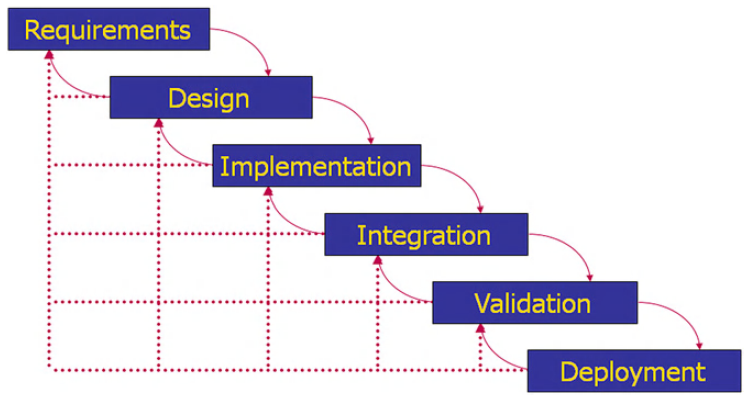
\includegraphics[width=0.9\linewidth]{waterfall.png}
	\caption{Modelo de desarrollo de software \textit{Waterfall}}
	\label{fig0001}
\end{figure}

\begin{figure}
	\centering
	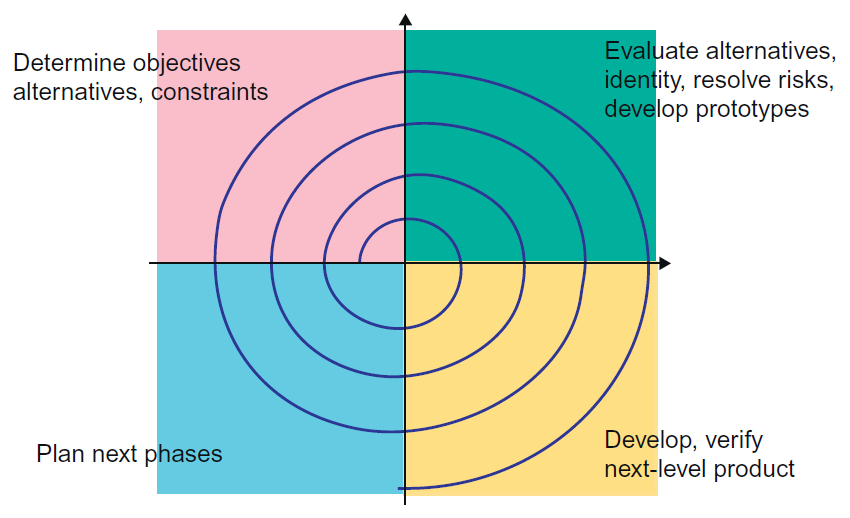
\includegraphics[width=0.9\linewidth]{espiral.png}
	\caption{Modelo de desarrollo de software \textit{Espiral}}
	\label{fig0002}
\end{figure}

\begin{figure}
	\centering
	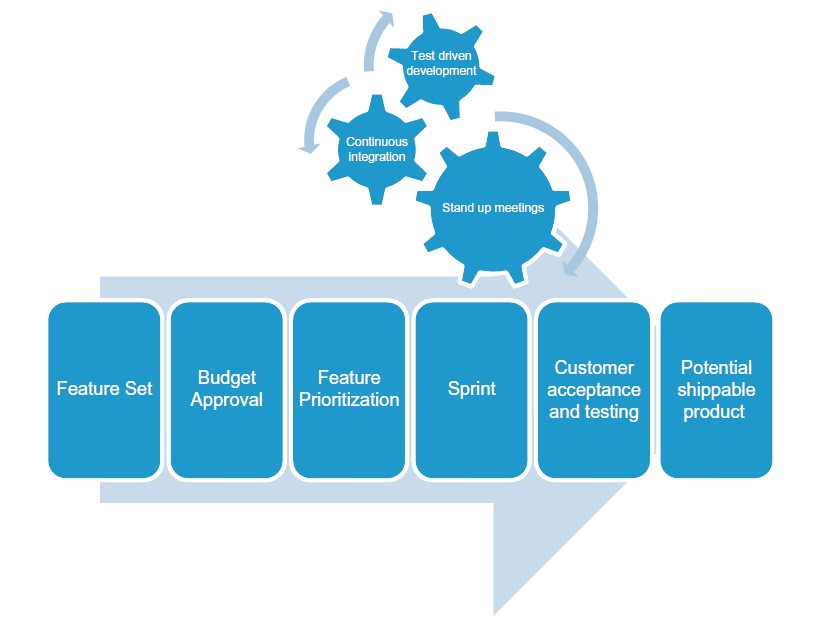
\includegraphics[width=0.9\linewidth]{agile.png}
	\caption{Modelo de desarrollo de software \textit{Agile}}
	\label{fig0003}
\end{figure}

La fases principales para el desarrollo de sistemas embebidos se pueden describir:
\begin{enumerate}
	\item \textbf{Definición del problema}: En esta fase se determina exactamente que quiere el cliente y el usuario. Esto incluye el desarrollo de un contrato con el cliente, dependiendo que tipo de producto esta siendo desarrollado. El objetivo de esta fase es especificar que producto de software se hará. Las dificultades incluyen: la solicitud del cliente por el producto incorrecto, el cliente no sabe sobre computación/software, lo cual limita la efectividad de esta fase, las especificaciones por lo regular son ambiguas, inconsistentes e incompletas.
	\item \textbf{Arquitectura/diseño}: La arquitectura se refiere a la selección de los elementos de arquitectónicos, sus interacciones, y las restricciones de aquellos elementos y sus interacciones necesarios para proporcionar un ambiente de trabajo con el cual satisfacer los requerimientos y servir como base para el diseño.  El diseño se refiere a la modularización y detalle de interfaz entre los elementos de diseño, sus algoritmos y procedimientos, y los tipos de datos necesarios para soportar la arquitectura y satisfacer los requerimientos. Durante la fase de arquitectura y diseño, el sistema es descompuesto en módulos de software con interfaces. Durante el diseño, el equipo de software desarrolla las especificaciones de los módulos (algoritmos y los tipos de datos),  manteniendo un récord de las decisiones de diseño y la trazabilidad, y especifica como los productos de software harán estas tareas. La dificultad principal durante esta fase incluye la falta de comunicación entre los diseñadores de módulos y terminan desarrollando un diseño que puede ser inconsistente, incompleto y ambiguo.
	\item \textbf{Implementación}: Durante esta fase el equipo de desarrollo implementa los módulos y componentes y verifica que cumplan las especificaciones. Los módulos se combinan de acuerdo con el diseño. Las implementaciones especifican como los productos del software hacen su trabajo. Algunas de las dificultades principales incluyen los errores de interacción entre los módulos y los errores de integración que pueden influenciar la calidad y la productividad.

	\item \textbf{Verificación y Validación(V\&V)}: Hay varias formas de V\&V. Una forma es el ``análisis''. El análisis puede ser en la forma de verificación estática, científica y formal y en revisiones informales. Las pruebas es una forma dinámica de V\&V. Esta forma de pruebas viene en la forma de una caja blanca (se tiene acceso al código) y de caja negra (no hay acceso al código). Las pruebas pueden ser estructurales o de comportamiento.Hay pruebas estándares para realizar dependiendo del producto a desarrollar.
	 
\end{enumerate}

Mas y mas desarrollo de software para sistemas embebidos se esta moviendo al desarrollo basado en componentes.Este tipo de desarrollo es aplicado generalmente para componentes de tamaño razonable y reutilización a través del sistema, que es una tendencia creciente en sistemas embebidos. Los desarrolladores aseguran que estos componentes son adaptables a contextos variantes y extienden la idea mas allá del código a otros artefactos desarrollados también. Esta técnica cambia la ecuación desde ``Integración, entonces Bajar al Hardware'' a ``Bajar al Hardware, entonces Implementar''.

\section{Definición formal de Sistemas Embebidos}

Se trata de un sistema de computación diseñado  para realizar una o algunas funciones dedicadas frecuentemente en un sistema de computación en tiempo real. Al contrario de lo que ocurre con los ordenadores de propósito general (como por ejemplo una computadora personal o PC) que están diseñados para cubrir un amplio rango de necesidades, los sistemas embebidos se diseñan para cubrir necesidades específicas.

\section{Historia}

\chapter{Aplicaciones con Angular 2}

Desde su creación hace ya más de 4 años, Angular ha sido el framework preferido por la mayoría de los desarrolladores Javascript. Este éxito ha provocado que los desarrolladores quieran usar el framework para más y más cosas.

De ser una plataforma para la creación de Web Apps, ha evolucionado como motor de una enorme cantidad de proyectos del ámbito empresarial y de ahí para aplicaciones en la Web Mobile Híbrida, llevando la tecnología al límite de sus posibilidades.

Es el motivo por el que comenzaron a detectarse problemas en Angular 1, o necesidades donde no se alcanzaba una solución a la altura de lo deseable. Son las siguientes.

\begin{itemize}
\item Javascript.-  Para comenzar encontramos problemas en la creación de aplicaciones debido al propio Javascript. Es un lenguaje con carácter dinámico, asíncrono y de complicada depuración. Al ser tan particular resulta difícil adaptarse a él, sobre todo para personas que están acostumbradas a manejar lenguajes más tradicionales como Java o C\#, porque muchas cosas que serían básicas en esos lenguajes no funcionan igualmente en Javascript.

\item Desarrollo del lado del cliente.- Ya sabemos que con Angular te llevas al navegador mucha programación que antes estaba del lado del servidor, comenzando por el renderizado de las vistas. Esto hace que surjan nuevos problemas y desafíos. Uno de ellos es la sobrecarga en el navegador, haciendo que algunas aplicaciones sean lentas usando Angular 1 como motor.
\end{itemize}

Por otra parte tenemos un impacto negativo en la primera visita, ya que se tiene que descargar todo el código de la aplicación (todas las páginas, todas las vistas, todas las rutas, componentes, etc), que puede llegar a tener un peso de megas. A partir de la segunda visita no es un problema, porque ya están descargados los scripts y cacheados en el navegador, pero para un visitante ocasional sí que representa un inconveniente grande porque nota que la aplicación tarda en cargar inicialmente.

Los intentos de implementar Lazy Load, o carga perezosa, en el framework en su versión 1.x no fueron muy fructíferos. Lo ideal sería que no fuese necesario cargar toda tu aplicación desde el primer instante, pero es algo muy difícil de conseguir en la versión precedente por el propio inyector de dependencias de Angular 1.x.

Otro de los problemas tradicionales de Angular era el impacto negativo en el SEO, producido por un renderizado en el lado del cliente. El contenido se inyecta mediante Javascript y aunque se dice que Google ha empezado a tener en cuenta ese tipo de contenido, las posibilidades de posicionamiento de aplicaciones Angular 1 eran mucho menores. Nuevamente, debido a la tecnología de Angular 1, era difícil de salvar.


Todos esos problemas, difíciles de solucionar con la tecnología usada por Angular 1, han sido los que han impulsado a sus creadores a desarrollar desde cero una nueva versión del framework. La nueva herramienta está pensada para dar cabida a todos los usos dados por los desarrolladores, llevar a Javascript a un nuevo nivel comparable a lenguajes más tradicionales, siendo además capaz de resolver de una manera adecuada las necesidades y problemas de la programación del lado del cliente.
\section{Aportaciones de Angular 2}


En la imagen de la  figura \ref{fig100}  puedes ver algunas de las soluciones aportadas en Angular 2.

\begin{figure}
	\centering
	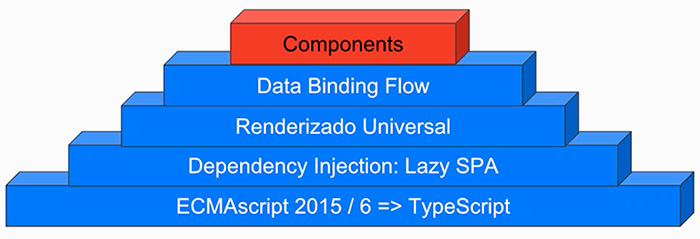
\includegraphics[width=0.9\linewidth]{angular2.jpg}
	\caption{Soluciones aportadas por Angular 2}
	\label{fig100}
\end{figure}


\subsection{TypeScript / Javascript} 
Como base hemos puesto a Javascript, ya que es el inicio de los problemas de escalabilidad del código. Ayuda poco a detectar errores y además produce con facilidad situaciones poco deseables.

Con ECMAscript 6 ya mejora bastante el lenguaje, facilitando la legibilidad del código y solucionando diversos problemas, pero todavía se le exige más. Ya puestos a no usar el Javascript que entienden los navegadores (ECMAscript 5), insertando la necesidad de usar un transpilador como Babel, podemos subir todavía un poco de nivel y usar TypeScript.
Angular 2 promueve el uso de TypeScript a sus desarrolladores. El propio framework está desarrollado en TypeScript, un lenguaje que agrega las posibilidades de ES6 y el futuro ES7, además de un tipado estático y ayudas durante la escritura del código, el refactoring, etc. pero sin alejarte del propio Javascript (ya que el código de Javascript es código perfectamente válido en TypeScript).

La sugerencia de usar TypeScript para desarrollar en Angular es casi una imposición porque la documentación y los generadores de código están pensados en TypeScript. Se supone que en futuro también estarán disponibles para Javascript, pero de momento no es así. De todos modos, para la tranquilidad de muchos, TypeScript no agrega más necesidad de procesamiento a las aplicaciones con Angular 2, ya que este lenguaje solamente lo utilizas en la etapa de desarrollo y todo el código que se ejecuta en el navegador es al final Javascript, ya que existe una transpilación previa.
 
 \subsection{Lazy SPA} 
Ahora el inyector de dependencias de Angular no necesita que estén en memoria todas las clases o código de todos los elementos que conforman una aplicación. En resumen, ahora con Lazy SPA el framework puede funcionar sin conocer todo el código de la aplicación, ofreciendo la posibilidad de cargar más adelante aquellas piezas que no necesitan todavía.

\subsection{Renderizado Universal} 
Angular nació para hacer web y renderizar en HTML en el navegador, pero ahora el renderizado universal nos permite que no solo se pueda renderizar una vista a HTML. Gracias a ésto, alguien podría programar una aplicación y que el renderizado se haga, por ejemplo, en otro lenguaje nativo para un dispositivo dado.

Otra cosa que permite el renderizado universal es que se use el motor de renderizado de Angular del lado del servidor. Es una de las novedades más interesantes, ya que ahora podrás usar el framework para renderizar vistas del lado del servidor, permitiendo un mejor potencial de posicionamiento en buscadores de los contenidos de una aplicación. Esta misma novedad también permite reducir el impacto de la primera visita, ya que podrás tener vistas "precocinadas" en el servidor, que puedes enviar directamente al cliente.

\subsection{Data Binding Flow}
Uno de los motivos del éxito de Angular 1 fue el data binding, pero éste tenía un coste en tiempo de procesamiento en el navegador, que si bien no penalizaba el rendimiento en todas las aplicaciones sí era un problema en aquellas más complejas. El flujo de datos ahora está mucho más controlado y el desarrollador puede direccionarlo fácilmente, permitiendo optimizar las aplicaciones. El resultado es que en Angular 2 las aplicaciones pueden llegar a ser hasta 5 veces más rápidas.

\subsection{Componentes}
La arquitectura de una aplicación Angular ahora se realiza mediante componentes. En este caso no se trata de una novedad de la versión 2, ya que en la versión de Angular 1.5 ya se introdujo el desarrollo basado en componentes.

Sin embargo, la componetización no es algo opcional como en Angular 1.5, sino es una obligatoriedad. Los componentes son estancos, no se comunican con el padre a no ser que se haga explícitamente por medio de los mecanismos disponibles, etc. Todo esto genera aplicaciones más mantenibles, donde se encapsula mejor la funcionalidad y cuyo funcionamiento es más previsible. Ahora se evita el acceso universal a cualquier cosa desde cualquier parte del código, vía herencia o cosas como el ``Root Scope'', que permitía en versiones tempranas de Angular modificar cualquier cosa de la aplicación desde cualquier sitio.

\section{Creando y configurando un proyecto}

En este paso nosotros:

\begin{itemize}
\item Crearemos una carpeta del proyecto
\item Agregar archivos de configuración y de definición de paquetes
\item Instalar Paquetes
\end{itemize}

\subsection{Crear una carpeta de proyecto}

\begin{lstlisting}[language=bash]
$ mkdir angular2-quickstart
$ cd    angular2-quickstart
\end{lstlisting}

\subsection{Agregar un archivo de definición de paquetes y de configuración}

Agregar los siguientes archivos de definición de paquetes y configuración a la carpeta del proyecto:

\begin{itemize}
\item \emph{package.json} . - Lista los paquetes de los cuales el proyecto depende y define algunos scripts útiles.
\item \emph{tsconfig.json}  .- Es el archivo de TypeScript de configuración del compilador.
\item \emph{typings.json} .- Identifica los archivos de definición de TypeScript.
\item \emph{systemjs.config.js} .- archivo de configuración de SystemJS.
\end{itemize}

\subsection{Instalar Paquetes }

Se instalan los paquetes listados en \emph{package.json} usando npm. Introducir el siguiente comando:

\begin{lstlisting}[language=bash]
$ npm install
\end{lstlisting}

Si la carpeta typings no se muestra  después de ejecutar npm install. Entonces, lo que tiene que ejecutarse es:

\begin{lstlisting}[language=bash]
$ npm run typing install
\end{lstlisting}

\subsection{Agregando las librerías y paquetes necesarios con \emph{npm}}

Los desarrolladores de aplicaciones utilizan el manejador de paquetes \emph{npm} para instalar librerías y paquetes que sus aplicaciones requieren. El equipo de Angular recomienda un conjunto inicial de paquetes especificado en las secciones \textbf{dependencies} y \textbf{devDependencies}.  Se han incluido un número de scripts \emph{npm} en el archivo propuesto \textbf{package.json} de la sub sección \ref{seccion:package}.

Muchos de los scripts de \emph{npm} se ejecutan de la siguiente manera: \textbf{npm run} seguido por el \textbf{nombre-script}. Algunos comandos (como el comando \textbf{start}) no necesitan la palabra clave \textbf{run}. Lo que los script realizan es:

\begin{itemize}
\item \textbf{npm start} .- ejecuta el compilador y el servidor al mismo tiempo, ambos en "\emph{watch mode}"
\item \textbf{npm run tsc} .- ejecuta el compilador TypeScript una vez.
\item \textbf{npm run tsc:w}.-  ejecuta el compilador TypeScript en \emph{watch mode}; el proceso se mantiene corriendo, esperando cambios del archivo TypeScript y recompilando cuando ve un cambio
\item \textbf{npm run lite} .- ejecuta el servidor lite, un servidor de archivos ligero con excelente soporte para aplicaciones Angular usando \textit{routing}.
 \item \textbf{npm run typings}.- ejecuta las herramientas \textit{typings} separadamente.
\item \textbf{npm run postinstall}.- llamado por \textit{npm} automáticamente después de instalar los paquetes completamente. Este script instala los archivos de definición TypeScript definidos en \emph{typings.json} 
\end{itemize}


\subsection{Archivo systemjs.config.js}

\begin{lstlisting}[language=bash]
/**
* System configuration for Angular 2 samples
* Adjust as necessary for your application needs.
 */
(function(global) {
  // map tells the System loader where to look for things
  var map = {
    'app':                        'app', // 'dist',
    '@angular':                   'node_modules/@angular',
    'angular2-in-memory-web-api': 'node_modules/angular2-in-memory-web-api',
    'rxjs':                       'node_modules/rxjs'
  };
  
  // packages tells the System loader how to load when no filename and/or no extension
  var packages = {
    'app':                        { main: 'main.js',  defaultExtension: 'js' },
    'rxjs':                       { defaultExtension: 'js' },
    'angular2-in-memory-web-api': { main: 'index.js', defaultExtension: 'js' },
  };
  
  var ngPackageNames = [
    'common',
    'compiler',
    'core',
    'forms',
    'http',
    'platform-browser',
    'platform-browser-dynamic',
    'router',
    'router-deprecated',
    'upgrade',
  ];
  
  // Individual files (~300 requests):
  function packIndex(pkgName) {
    packages['@angular/'+pkgName] = { main: 'index.js', defaultExtension: 'js' };
  }
  // Bundled (~40 requests):
  function packUmd(pkgName) {
    packages['@angular/'+pkgName] = { main: '/bundles/' + pkgName + '.umd.js', defaultExtension: 'js' };
  }
  // Most environments should use UMD; some (Karma) need the individual index files
  var setPackageConfig = System.packageWithIndex ? packIndex : packUmd;


   // Add package entries for angular packages
  ngPackageNames.forEach(setPackageConfig);
  var config = {
    map: map,
    packages: packages
  };
  System.config(config);
})(this);  

\end{lstlisting}

\subsection{Archivo package.json}
\label{seccion:package}

\begin{lstlisting}[language=java]

{

  "name": "angular2-quickstart",
  "version": "1.0.0",
  "scripts": {
    "start": "tsc && concurrently \"npm run tsc:w\" \"npm run lite\" ",
    "lite": "lite-server",
    "postinstall": "typings install",
    "tsc": "tsc",
    "tsc:w": "tsc -w",
    "typings": "typings"
  },
  "license": "ISC",
  "dependencies": {
    "@angular/common": "2.0.0-rc.5",
    "@angular/compiler": "2.0.0-rc.5",
    "@angular/core": "2.0.0-rc.5",
    "@angular/forms": "0.3.0",
    "@angular/http": "2.0.0-rc.5",
    "@angular/platform-browser": "2.0.0-rc.5",
    "@angular/platform-browser-dynamic": "2.0.0-rc.5",
    "@angular/router": "3.0.0-rc.1",
    "@angular/router-deprecated": "2.0.0-rc.2",
    "@angular/upgrade": "2.0.0-rc.5",
    "systemjs": "0.19.27",
    "core-js": "^2.4.0",
    "reflect-metadata": "^0.1.3",
    "rxjs": "5.0.0-beta.6",
    "zone.js": "^0.6.12",
    "angular2-in-memory-web-api": "0.0.15",
    "bootstrap": "^3.3.6"
  },
  "devDependencies": {
    "concurrently": "^2.0.0",
    "lite-server": "^2.2.0",
    "typescript": "^1.8.10",
    "typings": "^1.0.4"
  }
}
\end{lstlisting}

\subsection{Archivo tsconfig.json}


\begin{lstlisting}[language=java]

{
  "compilerOptions": {
    "target": "es5",
    "module": "commonjs",
    "moduleResolution": "node",
    "sourceMap": true,
    "emitDecoratorMetadata": true,
    "experimentalDecorators": true,
    "removeComments": false,
    "noImplicitAny": false
  }
}
\end{lstlisting}

\subsection{Archivo typings.json}

\begin{lstlisting}[language=java]

{
  "globalDependencies": {
    "core-js": "registry:dt/core-js#0.0.0+20160602141332",
    "jasmine": "registry:dt/jasmine#2.2.0+20160621224255",
    "node": "registry:dt/node#6.0.0+20160807145350"
  }
}
\end{lstlisting}

\section{Diseñando el primer componente en Angular}

Primero vamos a crear una carpeta para colocar nuestra aplicación y agregar un componente Angular simple.

\subsection{Crear una subcarpeta de la aplicación}
 Crear una carpeta en el directorio raíz para allí colocar todos los archivos de la aplicación.
 \begin{lstlisting}[language=bash]
 $ mkdir app
 \end{lstlisting}

\subsection{Crear el archivo de componente}

Se crea el archivo \textbf{app/app.component.ts} en el nuevo directorio creado con el siguiente contenido:
\begin{lstlisting}[language=java]
import { Component } from '@angular/core';
@Component({
  selector: 'my-app',
  template: '<h1>My First Angular 2 App</h1>'
})
export class AppComponent { }
\end{lstlisting}

Cada aplicación angular tiene al menos un componente raíz, convencionalmente llamado \textbf{\textit{AppComponent}}, que contiene la experiencia del usuario. Los componentes son los bloques fundamentales en las aplicaciones Angular. Un componente controla una parte de la pantalla- una vista- a través de los template asociados.

La estructura de cada componente contiene lo siguiente:

\begin{itemize}
\item Una o más sentencias \textit{\textbf{import}} para la referencia a las librerías u objetos de lo que se necesite
\item Un \textit{\textbf{@Component decorator}} que le dice a Angular que template usar y como crear el componente
\item A \textit{\textbf{component class}} que controla la apariencia y comportamiento de una vista a través de su template.
\end{itemize}

\subsubsection{Import}

Las aplicaciones Angular son modulares. Consisten de muchos archivos cada uno dedicado a un propósito. Angular en si mismo en modular. Es una colección de módulos de librerías cada uno hecho de varios módulos a su vez. 

Cuando necesitamos algo de un módulo o librería, la importamos. En este ejemplo importamos \textit{Angular 2 core} a nuestro componente y se puede acceder con el decorador \textit{\textbf{@Component}}.

\begin{lstlisting}[language=java]
import { Component } from '@angular/core';
\end{lstlisting}

\subsubsection{@Component decorator}

Component es una función decoradora que toma un objeto \textit{metadata} como argumento. Aplicamos esta función a la clase componente colocándole de prefijo a la función el símbolo \textbf{@} invocándola con el objeto \textit{metadata}.

\textit{\textbf{@Component}} es un decorador que nos permite asociar\textit{ metadata }con una clase componente. Los\textit{ metadata} le dicen a Angular como crear y usar este componente.

\begin{lstlisting}[language=java]
@Component({
  selector: 'my-app',
  template: '<h1>My First Angular 2 App</h1>'
})
\end{lstlisting}


Este objeto metadata particular tiene dos campos, un \textit{selector} y un \textit{template}.

El \textbf{selector} especifica un simple \textbf{selector} CSS para un elemento HTML que representa el componente. Los elementos para este componente se llaman \textit{my-app}. Angular crea y despliega una instancia de nuestro \textit{\textbf{AppComponent}} en donde encuentra un elemento \textit{my-app} en el archivo HTML.

El template especifica los formatos de los componentes, escrito en una forma mejorada de HTML que le dice a Angular como desplegar este componente. En este ejemplo nuestro template es una simple linea de HTML que anuncia "My First Angular 2 App". Un template mas avanzado puede contener enlaces de datos a las propiedades de los componentes y puede identificar otros componentes de aplicaciones los cuales tiene sus propios templates. Estos templates pueden identificar todavía otros componentes. De esta forma una aplicación Angular se convierte a un árbol de componentes.   

\subsection{Component class}

En el fondo del archivo hay una clase vacía que no hace nada llamada
\textbf{AppComponent}

\begin{lstlisting}[language=bash]
$ export class AppComponent { }
\end{lstlisting}

Cuando estamos listos para construir una aplicación, podemos expandir esta clase con propiedades y aplicaciones lógicas. Nuestra \textit{\textbf{AppComponent}} esta vacía porque no se necesita nada particular.
Se exporta \textit{\textbf{AppComponent}} de tal forma que podemos importarlo en cualquier lugar de nuestra aplicación, como se verá cuando se cree el archivo \textbf{app.module.ts}.

\section{creando app.module.ts}
Se crean aplicaciones Angular estrechamente relacionadas con bloques de funcionalidad con módulos angular. Cada aplicación requiere al menos un módulo, el módulo raíz, que se llama \textbf{AppModule} por convención.


Crear un archivo app/app.module.ts con el siguiente contenido:

\begin{lstlisting}[language=java]
import { NgModule }      from '@angular/core';
import { BrowserModule } from '@angular/platform-browser';

import { AppComponent }  from './app.component';

@NgModule({
  imports:      [ BrowserModule ],
  declarations: [ AppComponent ],
  bootstrap:    [ AppComponent ]
})
export class AppModule { }
\end{lstlisting}

Se pasan metadata a la función decoradora NgModule

\begin{itemize}
\item imports .- los otros módulos que exportan material que necesitamos en este módulo. Casi cada aplicación módulo raíz debe importar el \textbf{BrowserModule}.
\item declarations .- Componentes y directivas que pertenecen a este módulo
\item bootstrap .- identifica el componente raíz que angular. La palabra inglesa bootstrapping es generalmente un término utilizado para describir el arranque, o proceso de inicio de cualquier ordenador. Suele referirse al programa que arranca un sistema operativo como por ejemplo GRUB, LiLo (utilizados en sistemas GNU/Linux, por ejemplo), BCD o NTLDR (utilizados en sistemas Windows). Se ejecuta tras el proceso POST (power-on-self-test) del BIOS. También es llamado «Boot loader» (cargador de inicio).
\end{itemize}

Importamos nuestra \textbf{app.component.ts} y se agrega tanto a \textbf{declarations} y al arreglo \textbf{bootstrap}.
 
Agregamos el BrowserModule desde @angular/platform-browser al arreglo import. Este es el modulo Angular que contiene todo lo que necesitamos para correr nuestra aplicación en el navegador.

\section{Agregar main.ts}

Ahora es necesario decirle a Angular que cargue el modulo de aplicación. Para ello se crea el archivo \textbf{app/main.ts} con el siguiente contenido:

\begin{lstlisting}[language=java]
import { platformBrowserDynamic } from '@angular/platform-browser-dynamic';

import { AppModule } from './app.module';

platformBrowserDynamic().bootstrapModule(AppModule);
\end{lstlisting}

Se importan dos cosas necesarias para cargar la aplicación:


\begin{itemize}
\item La función Navegador Angular  \textbf{platformBrowserDynamic}
\item El módulo de aplicación \textbf{AppModule}
\end{itemize}

Entonces se llama \textbf{platformBrowserDynamic().bootstrapModule} con \textbf{AppComponent}

\section{El Bootstraping es específico de la plataforma }

Es importante puntualizar que importamos la función \textbf{platformBrowserDynamic} desde \textbf{@angular/platform-browser-dynamic} y no desde \textbf{@angular/core}. Bootstrapping no esta en el core porque no hay una manera simple para arrancar la aplicación. Muchas aplicaciones que corren en un navegador llaman a la función bootstrap desde esta librería. Pero es posible cargar un módulo en un ambiente diferente. Es posible cargar desde un dispositivo con Apache Cordova o NativeScript. 

\section{Agregar un archivo index.html}

En la carpeta raíz del proyecto se crea un archivo index.html con el siguiente contenido:


\begin{lstlisting}[language=html]
<html>
  <head>
    <title>Angular 2 QuickStart</title>
    <meta charset="UTF-8">
    <meta name="viewport" content="width=device-width, initial-scale=1">
    <link rel="stylesheet" href="styles.css">
    <!-- 1. Load libraries -->
     <!-- Polyfill(s) for older browsers -->
    <script src="node_modules/core-js/client/shim.min.js"></script>
    <script src="node_modules/zone.js/dist/zone.js"></script>
    <script src="node_modules/reflect-metadata/Reflect.js"></script>
    <script src="node_modules/systemjs/dist/system.src.js"></script>
    <!-- 2. Configure SystemJS -->
    <script src="systemjs.config.js"></script>
    <script>
      System.import('app').catch(function(err){ console.error(err); });
    </script>
  </head>
  <!-- 3. Display the application -->
  <body>
    <my-app>Loading...</my-app>
  </body>
</html>
\end{lstlisting}

El archivo index.html define la pagina web que alojará la aplicación. Las secciones del archivo HTML son:

\begin{itemize}
\item Las librerias de JavaScript
\item El archivo de configuración para \textbf{SystemJS}, y el script donde se importa y ejecuta el módulo de la \textit{app} que llama al archivo \textit{main} 
\item El tag \textbf{<my-app>} en el \textbf{<body>} que es donde nuestro \textit{app} vive.
\end{itemize}

\subsection{Agregando algo de estilo}
Los estilos no son esenciales pero son agradables, y el archivo \textbf{index.html} supone que tenemos un archivo de estilos llamado \textbf{style.css}.

Crear el archivo \textbf{style.css} en la carpeta raíz del proyecto para poder cargarlo con el código mínimo que se muestra a continuación:


\begin{lstlisting}[language=html]
/* Master Styles */
h1 {
  color: #369;
  font-family: Arial, Helvetica, sans-serif;
  font-size: 250%;
}
h2, h3 {
  color: #444;
  font-family: Arial, Helvetica, sans-serif;
  font-weight: lighter;
}
body {
  margin: 2em;
}
\end{lstlisting}


\section{Construir y ejecutar la app}

En una terminal ejecutar el siguiente comando:

\begin{lstlisting}[language=html]
npm start
\end{lstlisting}
 El comando anterior ejecuta dos procesos en paralelo:
 
 \begin{itemize}
\item El compilador TypeScript en \textbf{watch mode}
\item Un servidor estático llamado \textbf{lite-server} que carga \textbf{index.html} en un navegador y refresca el navegador cuando el archivo cambia
\end{itemize}

En la figura \ref{fig101} se puede ver la arquitectura general de un proyecto en angular 2.

\begin{figure}
	\centering
	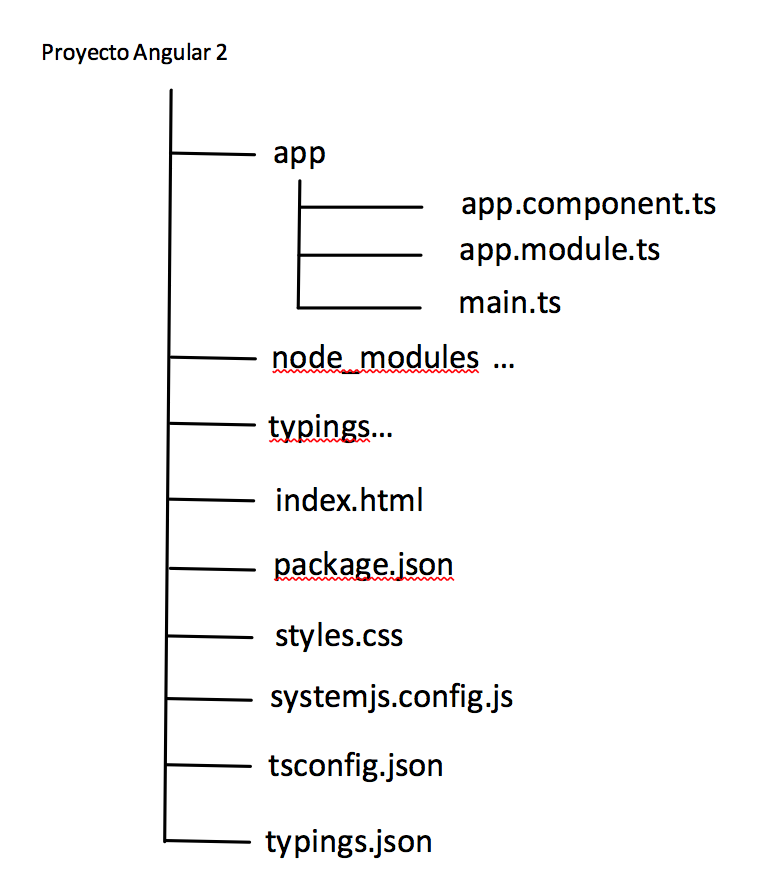
\includegraphics[width=0.5\linewidth]{angular.png}
	\caption{Sistema de archivos de Angular 2}
	\label{fig101}
\end{figure}

\section{Diseñando una aplicación de ejemplo}

Suponiendo que deseamos agregar datos a nuestra app, para ello agregamos dos componentes a nuestro AppComponent, como \textit{título} y \textit{heroe}.


\begin{lstlisting}[language=html]
export class AppComponent {
  titulo = 'Listado de SuperHeroes';
  heroe = 'Superman';
  }
  \end{lstlisting}


Después se actualiza el formato en la decoración \textit{@Component} con enlace de datos a estas nuevas propiedades


\begin{lstlisting}[language=html]
template: '<h1>{{titulo}}</h1><h2>Detalles del Super Heroe {{heroe}} </h2>'
  \end{lstlisting}
  
  El navegador mostrará ahora el nombre del super héroe. Las dobles llaves le dicen que a nuestra aplicación leer las propiedades \textit{titulo} y \textit{heroe} desde los componentes.





\bibliographystyle{acm}
\bibliography{../bibliografia}

\end{document}